\begin{frame}{Video Encoding Frames}
  \begin{figure}
    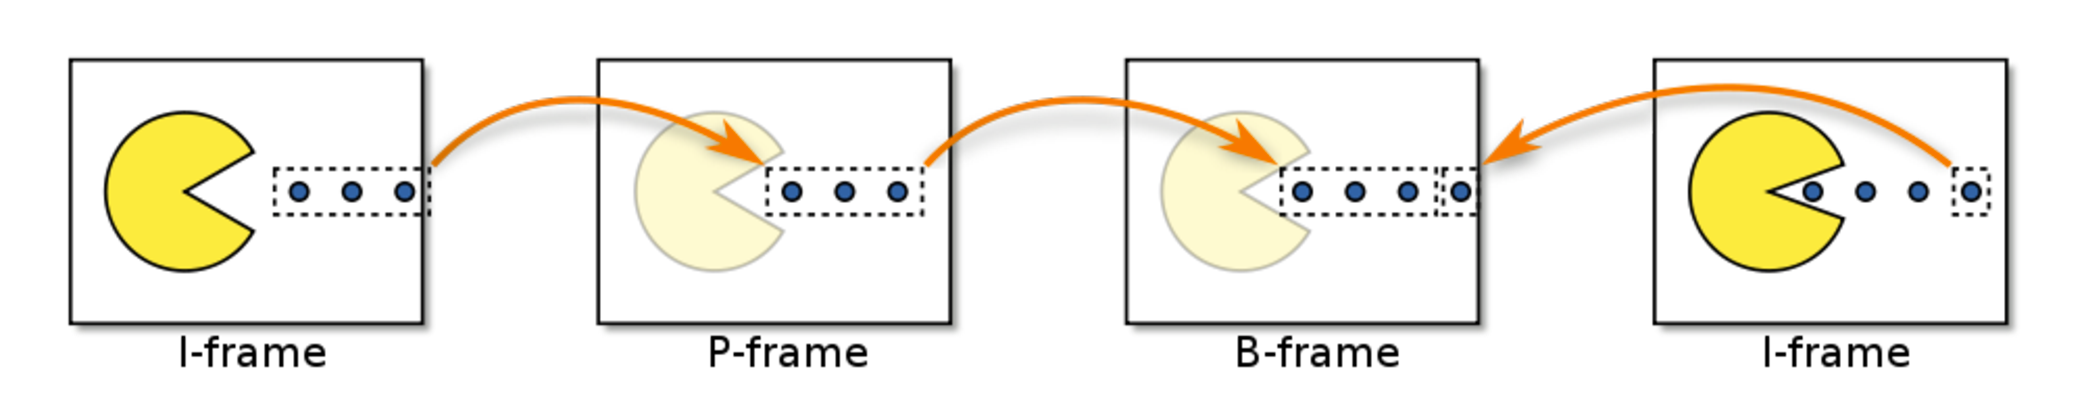
\includegraphics[width=\textwidth]{figures/video-frames.pdf}
    \caption{PC: https://en.wikipedia.org/wiki/Video\_compression\_picture\_types}
  \end{figure}

  \begin{itemize}
  \item \textbf{I-frames} are the least compressible but don't require other
    video frames to decode. I-frames are further compressed with
    quantization.
  \item \textbf{P-frames} can use data from previous frames to decompress
    and are more compressible than I-frames.
  \item \textbf{B-frames} can use both previous and forward frames for data
    reference to get the highest amount of data compression (not an option
    in live streaming).
  \end{itemize}
\end{frame}

\begin{frame}{Evaluation: Resource Allocation for Multiple Applications}
  \centering
  \begin{figure}
    \centering
    \begin{subfigure}[t]{0.7\columnwidth}
      \centering
      
\includegraphics[width=\textwidth]{figures/multitask-legend.pdf}
    \end{subfigure}
    \\
    \vspace{1em}
    \begin{subfigure}[t]{0.45\columnwidth}
      \centering
      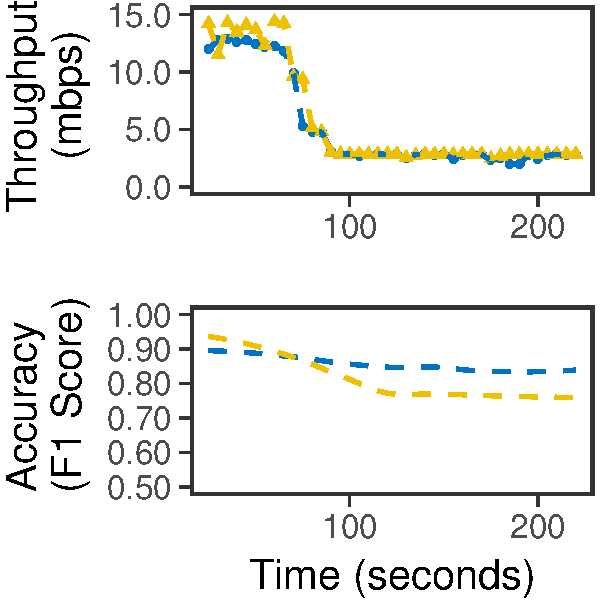
\includegraphics[width=\textwidth]{figures/multitask-left.pdf}
      \caption{Resource Fairness}
      \label{fig:eq-bw}
    \end{subfigure}
    \hfill
    \begin{subfigure}[t]{0.45\columnwidth}
      \centering
      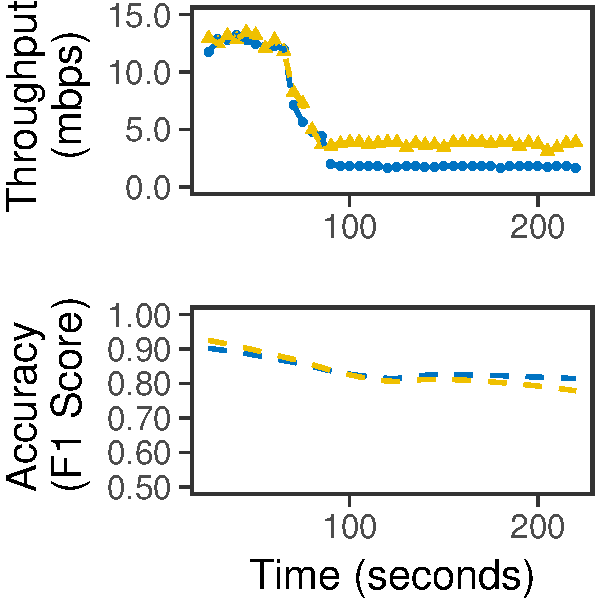
\includegraphics[width=\textwidth]{figures/multitask-right.pdf}
      \caption{Utility Fairness}
      \label{fig:eq-acc}
    \end{subfigure}
  \end{figure}
\end{frame}

\begin{frame}{Bandwidth Fluctuations (Cellular)}
  \hypertarget{cellular-variation}{}
  \begin{figure}
    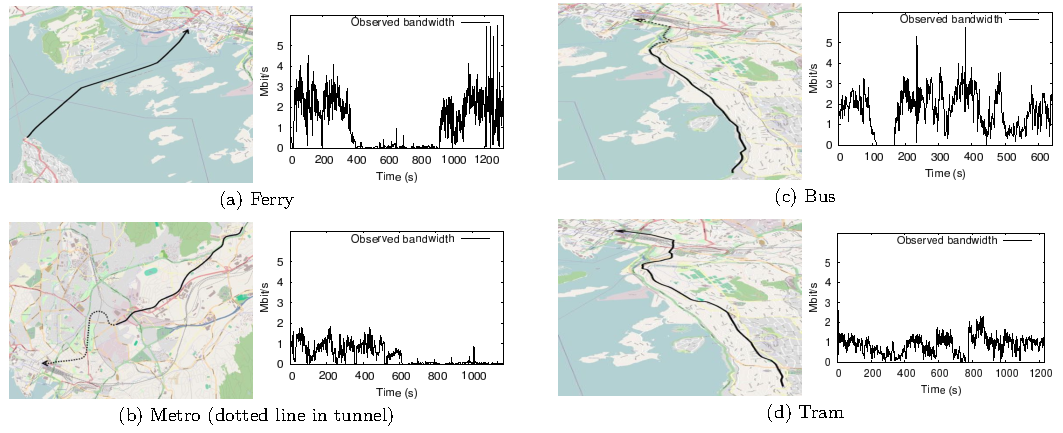
\includegraphics[width=\textwidth]{figures/bandwidth-cellular.pdf}
    \caption{Riiser, Haakon, et al. "A comparison of quality scheduling in
      commercial adaptive HTTP streaming solutions on a 3G network."
      Proceedings of the 4th Workshop on Mobile Video. ACM, 2012.}
  \end{figure}
\end{frame}

\begin{frame}{Bandwidth Fluctuations (WiFi)}
  \footnotesize
  \begin{figure}
    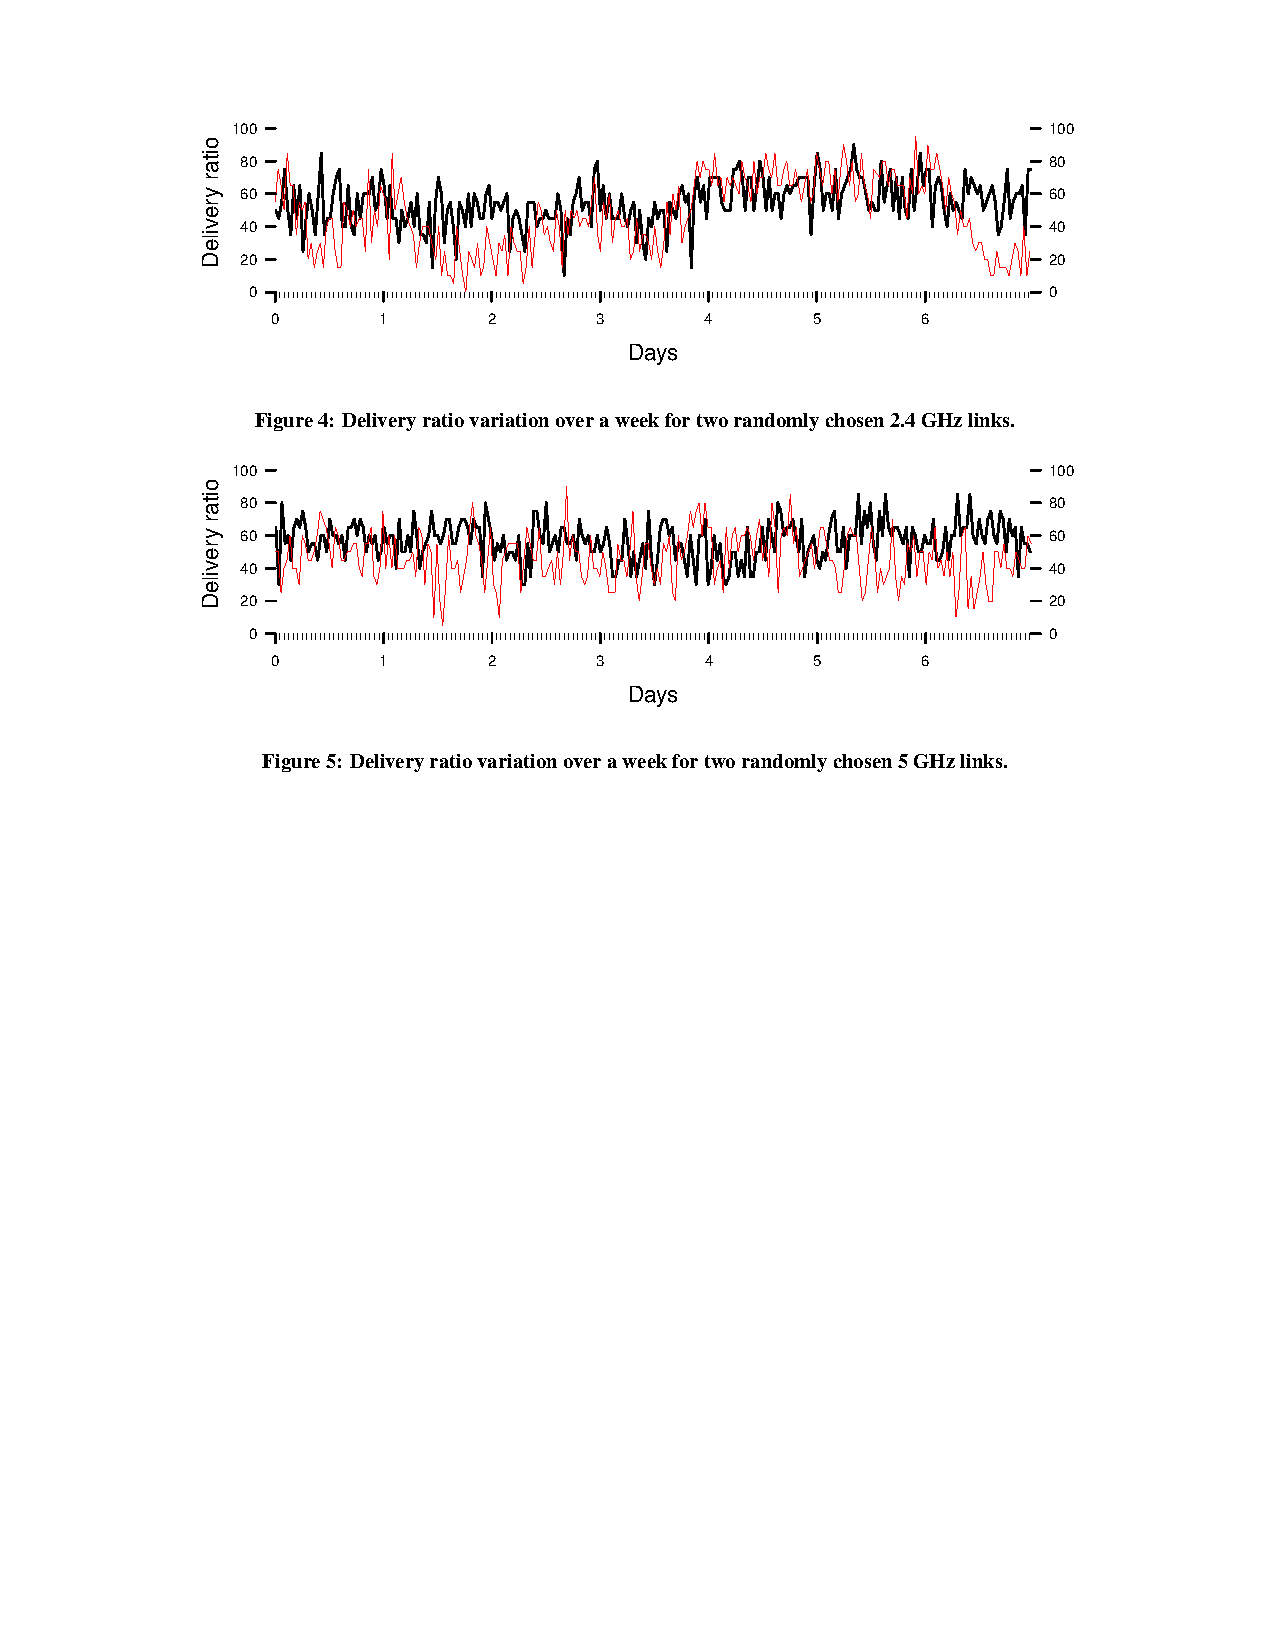
\includegraphics[width=0.7\textwidth]{figures/bandwidth-wifi.pdf}
    \caption{Biswas et al, Cisco Meraki, Large-scale Measurements of Wireless
      Network Behavior, SIGCOMM'15. Two randomly chosen links.}
  \end{figure}

  \hyperlink{aws-variation}{Continue with the main slides}.
\end{frame}

\begin{frame}{Augmented Reality}
  \begin{itemize}
  \item Training and testing data characteristics
    \begin{itemize}
    \item 1920x1080 resolution with 30 FPS
    \item training: 707 frames (23.5 seconds), testing: 1384 frames (46 seconds)
    \end{itemize}
  \item Object Recognition
    \begin{itemize}
    \item Darknet: Open Source Neural Networks in C
    \item Developed by Joseph Redmon, "Do whatever you want with it" license
    \item It supports CPU/GPU
    \item In this work, I am using a pre-trained model with Coco dataset
    \end{itemize}
  \item Other systems such as TensorFlow, Caffe would also work
  \end{itemize}
\end{frame}

\begin{frame}{IOU and F1}
  \hypertarget{iou-f1}{}
  \vspace{1em}
  \begin{columns}
    \column{0.5\textwidth}
    Positive if intersection over union (IOU) larger than 0.5.

    \[
      \text{IOU} = \frac{\text{Area of Intersection}}{\text{Area of Union}}
    \]

    \begin{figure}
      \begin{subfigure}{0.3\textwidth}
        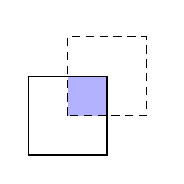
\begin{tikzpicture}
          \fill[color=blue!30] (0.5, 0.5) rectangle (1, 1);
          \node[draw=none] () at (1.5, 1.5) {};
          \draw (0, 0) rectangle (1, 1);
          \draw[densely dashed] (0.5, 0.5) rectangle (1.5, 1.5);
        \end{tikzpicture}
        \caption{IOU=0.14}
      \end{subfigure}
      \begin{subfigure}{0.3\textwidth}
        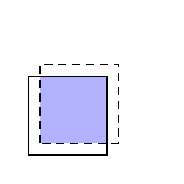
\begin{tikzpicture}
          \fill[color=blue!30] (0.15, 0.15) rectangle (1, 1);
          \node[draw=none] () at (1.5, 1.5) {};
          \draw (0, 0) rectangle (1, 1);
          \draw[densely dashed] (0.15, 0.15) rectangle (1.15, 1.15);
        \end{tikzpicture}
        \caption{IOU=0.57}
      \end{subfigure}
      \begin{subfigure}{0.3\textwidth}
        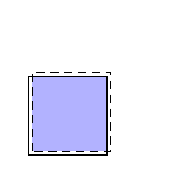
\begin{tikzpicture}
          \fill[color=blue!30] (0.05, 0.05) rectangle (1, 1);
          \node[draw=none] () at (1.5, 1.5) {};
          \draw[densely dashed] (0.05, 0.05) rectangle (1.05, 1.05);
          \draw (0, 0) rectangle (1, 1);
        \end{tikzpicture}
        \caption{IOU=0.82}
      \end{subfigure}
    \end{figure}

    \column{0.5\textwidth}
    
    F1 is the harmonic mean of precision and recall:

    \begin{table}
      \centering
      \begin{tabular}{| c | c | c |}
        \hline
        & P & N \\
        \hline
        Y & True Positive & False Positive \\
        \hline
        N & True Positive & False Positive \\
        \hline
      \end{tabular}
    \end{table}

    \begin{equation*}
      \begin{split}
        \text{Precision} &= \frac{\text{true positive}}{\text{all positive}} \\
        \text{Recall} &= \frac{\text{true positive}}{\text{all detection}} \\
        \text{F1} &= \frac{2}{\frac{1}{\text{Recall}} + \frac{1}{\text{Precision}}}
      \end{split}
    \end{equation*}
  \end{columns}
\end{frame}

%%% Local Variables:
%%% mode: latex
%%% TeX-master: "talk"
%%% TeX-engine: xetex
%%% End:
